\section{Analiza Wyników i Działania Systemu}
\label{sec:Analiza_wynikow}

\subsection{Cel analizy i kryteria oceny}

Rozdział ma charakter porównawczy i zestawia ze sobą dwa podejścia do rozwijania modelu AI: manualne oraz zautomatyzowane CI/CD.

Aby porównanie było jednoznaczne, analizę przeprowadzono w sześciu wymiarach:
\begin{itemize}
  \item nakład pracy człowieka i całkowity czas realizacji cyklu
  \item jakość modelu (Dice, IoU) i skuteczność bramki jakości,
  \item koszty infrastruktury,
  \item zużycie zasobów,
  \item ryzyko błędu ludzkiego
  \item skalowalność procesu.
\end{itemize}

\subsection{Metodologia porównania}

Porównano dwa scenariusze realizujące ten sam cel biznesowy (dodanie nowych danych i dostarczenie działającego modelu):
\begin{enumerate}
  \item \textbf{Podejście ręczne} --- inżynier ręcznie wykonuje kolejne kroki: walidację danych, trening, ocenę metryk, decyzję o promocji modelu i wdrożenie.
  \item \textbf{Podejście zautomatyzowane (zrealizowany pipeline)} --- operator dostarcza dane przez \texttt{git push}, a dalszy przebieg realizują skrypty i workflow.
\end{enumerate}

Utrzymanie porównywalnego środowiska narzędziowego w obu podejściach było kluczowe. Pozwala przypisać różnice w nakładzie pracy i ryzyku błędu automatyzacji procesu, a nie zmianie technologii. Dokładniejsze wskazanie granicy między podejściami ułatwia poniższe zestawienie:
\begin{itemize}
  \item \textbf{Narzędzia wspólne dla obu podejść:} EC2 (środowisko obliczeniowe), MLflow (śledzenie eksperymentów, metryk i wersji modeli), k3s z Helm (wdrożenie), Docker (konteneryzacja API).
  \item \textbf{Narzędzia wyłącznie dla podejścia zautomatyzowanego:} GitHub Actions (orkiestracja pipeline), DVC (wersjonowanie \textit{danych treningowych} i synchronizacja z S3), hook \texttt{pre-push} Git (automatyczne tworzenie gałęzi danych), Terraform (infrastruktura jako kod).
\end{itemize}

Porównanie obejmuje sześć wymiarów:
\begin{itemize}
  \item \textbf{Nakład pracy człowieka i czas całkowity} (podsekcja~\ref{subsec:czasy}),
  \item \textbf{Jakość modelu} (podsekcja~\ref{subsec:metryki}),
  \item \textbf{Koszty infrastruktury i obsługi} (podsekcja~\ref{subsec:koszty}),
  \item \textbf{Zużycie zasobów} (podsekcja~\ref{subsec:zasoby}),
  \item \textbf{Ryzyko błędu ludzkiego} (podsekcje~\ref{subsubsec:stabilnosc}).
  \item \textbf{skalowalność procesu} (podsekcje~\ref{subsubsec:skalowalnosc}).
\end{itemize}

\textbf{Istotne ograniczenie metodologiczne:} czasy dla podejścia ręcznego mają charakter szacunkowy i zostały określone na podstawie doświadczeń zdobytych podczas realizacji projektu oraz analizy poszczególnych etapów procesu. Czasy podejścia zautomatyzowanego pochodzą z logów GitHub Actions i stanowią rzeczywisty pomiar czasu wykonania.

\subsection{Czasy wykonania i nakład pracy człowieka}
\label{subsec:czasy}

\begin{table}[H]
\centering
\caption{Porównanie nakładu pracy człowieka i czasu realizacji cyklu}
\label{tab:czasy}
\begin{tabular}{|l|r|r|}
\hline
\textbf{Etap} & \textbf{Ręczny} & \textbf{Zautomatyzowane CI/CD} \\
\hline
Przygotowanie i upload danych & $\sim$30 min & $\sim$10 min \\
Walidacja danych & $\sim$30 min & automatyczna \\
Trening modelu & $\sim$3 h & automatyczny \\
Ocena jakości i decyzja wdrożeniowa & $\sim$15 min & automatyczna \\
Wdrożenie & $\sim$45 min & automatyczne \\
\hline
\textbf{Nakład człowieka łącznie} & $\sim$5 h & $\sim$20 min \\
\textbf{Całkowity czas cyklu} & $\sim$5 h & $\sim$4 h \\
\hline
\end{tabular}
\end{table}

Wynik oznacza redukcję aktywnego czasu inżyniera o około \textbf{93\%} (z 300 min do 20 min) na jeden cykl. Jednocześnie całkowity czas cyklu został skrócony o około \textbf{20\%}, ponieważ głównym składnikiem pozostaje sam trening modelu. Zakładając pewną niedokładność oszacowań, wyniki nadal pozostają jednoznaczne: automatyzacja znacząco redukuje nakład pracy człowieka i skraca czas realizacji procesu.

Kluczowe jest rozróżnienie między \textbf{nakładem pracy człowieka} a \textbf{całkowitym czasem realizacji}. W podejściu ręcznym obie wartości są praktycznie tożsame, ponieważ operator uczestniczy we wszystkich etapach. W podejściu zautomatyzowanym człowiek dostarcza dane, a następnie pipeline działa bez jego udziału co jest ogromną zaletą dla podejścia zautomatyzowanego.

W praktyce ta różnica może się dodatkowo powiększyć przez fakt, że cykl manualny obejmuje kilkanaście interwencji: uruchomienie środowiska, trening, monitorowanie logów, ocenę metryk, rejestrację modelu, aktualizację konfiguracji wdrożenia i weryfikację działania po deploymencie. Każdy etap jest potencjalnym źródłem błędu. W pipeline CI/CD większość tych kroków jest wykonywana automatycznie i audytowalnie.

\subsection{Jakość modeli i skuteczność bramki jakości}
\label{subsec:metryki}

Poniższe wykresy i tabela nr~\ref{tab:metryki} przedstawiają metryki zarejestrowane w MLflow dla kolejnych wersji modelu.

\begin{figure}[H]
 \centering
 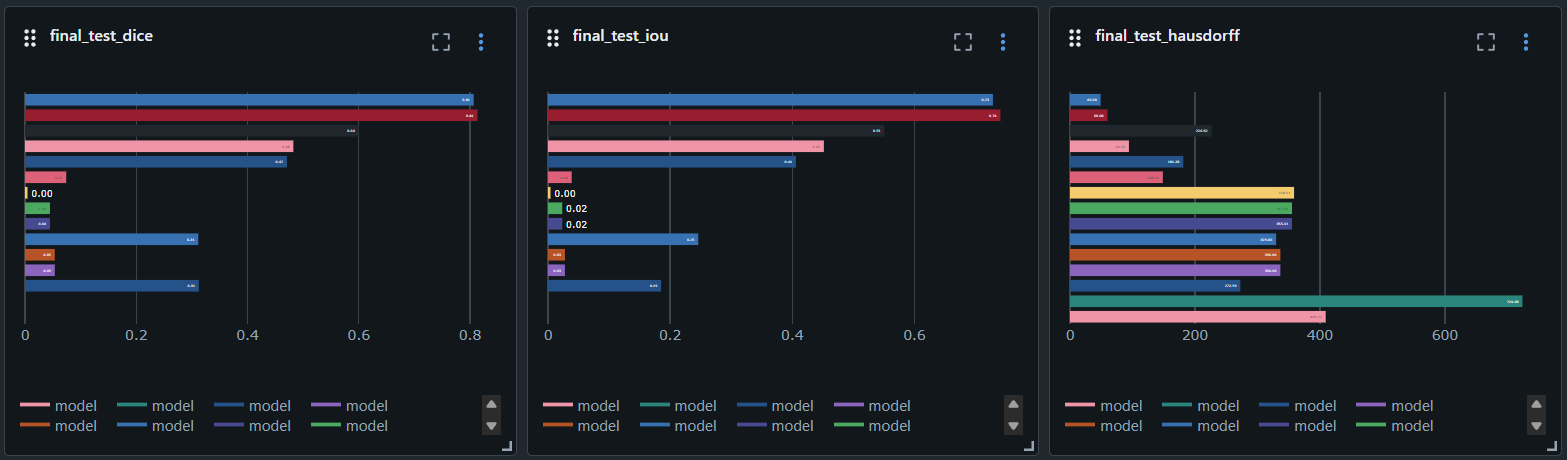
\includegraphics[width=\linewidth]{img/07_analiza_wynikow_i_dzialanie_systemu/mlfow_models_metrics_all.png}
 \caption{Metryki jakości modelu w interfejsie MLflow}
 \label{fig:mlflow-metrics-all}
\end{figure}

\begin{table}[H]
\centering
\caption{Metryki jakości modelu dla kolejnych wersji}
\label{tab:metryki}
\begin{tabular}{|l|c|c|c|}
\hline
\textbf{Wersja modelu} & \textbf{Dice} & \textbf{IoU} & \textbf{Hausdorff} \\
\hline
v21  & 0{,}8067 & 0{,}7286 & 49{,}0034 \\
v20  & 0{,}8134 & 0{,}7409 & 59{,}9987 \\
v18  & 0{,}5998 & 0{,}5508 & 226{,}5247 \\
v16  & 0{,}4825 & 0{,}4518 & 94{,}3321 \\
v14  & 0{,}4710 & 0{,}4060 & 181{,}2840 \\
v13  & 0{,}0741 & 0{,}0388 & 148{,}5599 \\
v12  & 0{,}0042 & 0{,}0021 & 358{,}6141 \\
v11  & 0{,}0449 & 0{,}0233 & 355{,}3105 \\
v10  & 0{,}0449 & 0{,}0233 & 355{,}3105 \\
v9   & 0{,}3116 & 0{,}2461 & 329{,}8586 \\
v8   & 0{,}0536 & 0{,}0278 & 336{,}6613 \\
v7   & 0{,}0536 & 0{,}0278 & 336{,}6613 \\
v5   & 0{,}3125 & 0{,}1852 & 272{,}5949 \\
v3   & $3{,}5689\cdot 10^{-10}$ & $3{,}5689\cdot 10^{-10}$ & 724{,}0773 \\
v1   & $3{,}5386\cdot 10^{-10}$ & $3{,}5386\cdot 10^{-10}$ & 409{,}2163 \\
\hline
\end{tabular}
\end{table}

Dane przedstawione w powyższej tabeli wskazują, że wszystkie modele były poprawnie rejestrowane niezależnie od osiągniętych metryk jakościowych.

\begin{table}[H]
\centering
\caption{Wersje modelu awansowane do etapu Production}
\label{tab:metryki-production}
\begin{tabular}{|l|c|c|c|}
\hline
\textbf{Wersja modelu} & \textbf{Dice} & \textbf{IoU} & \textbf{Hausdorff} \\
\hline
v20  & 0{,}8134 & 0{,}7409 & 59{,}9987 \\
v18  & 0{,}5998 & 0{,}5508 & 226{,}5247 \\
v16  & 0{,}4825 & 0{,}4518 & 94{,}3321 \\
v14  & 0{,}4710 & 0{,}4060 & 181{,}2840 \\
v9   & 0{,}3116 & 0{,}2461 & 329{,}8586 \\
v5   & 0{,}3125 & 0{,}1852 & 272{,}5949 \\
v3   & $3{,}5689\cdot 10^{-10}$ & $3{,}5689\cdot 10^{-10}$ & 724{,}0773 \\
v1   & $3{,}5386\cdot 10^{-10}$ & $3{,}5386\cdot 10^{-10}$ & 409{,}2163 \\
\hline
\end{tabular}
\end{table}

\begin{figure}[H]
 \centering
 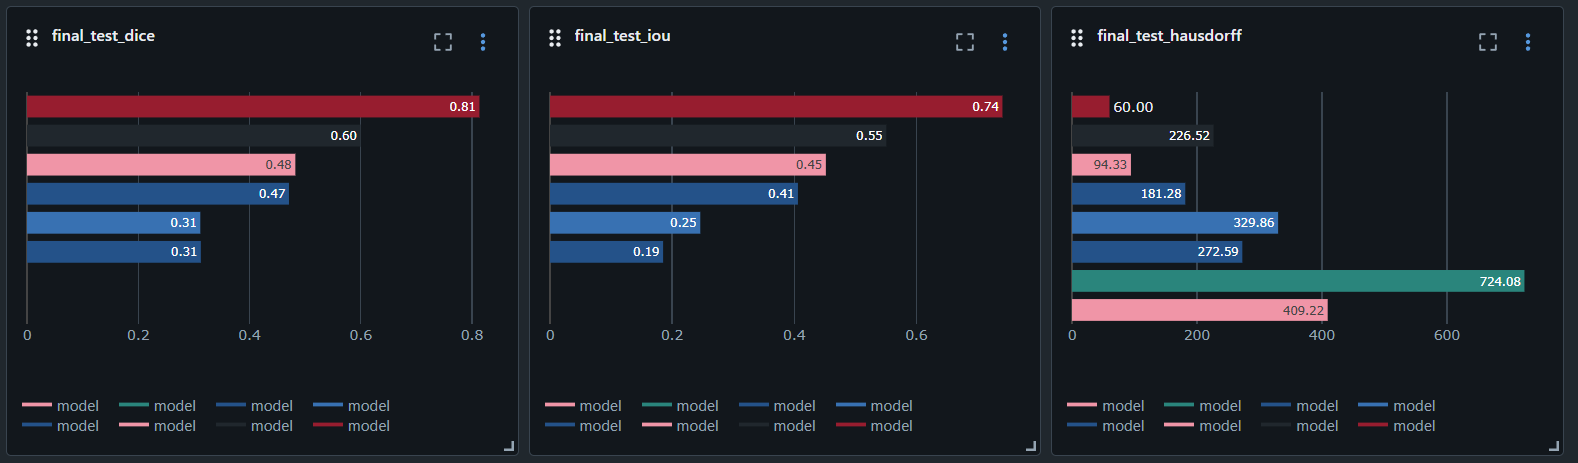
\includegraphics[width=\linewidth]{img/07_analiza_wynikow_i_dzialanie_systemu/mlflow_models_metrics_production.png}
 \caption{Rejestr modeli MLflow --- widok wersji ze stadium Production}
 \label{fig:mlflow-metrics-production}
\end{figure}
\mbox{}\\
Analiza całego zbioru wersji potwierdza poprawność mechanizmu kontroli jakości. Wszystkie przebiegi zostały zarejestrowane, natomiast do etapu \textit{Production} awansowały wyłącznie wersje spełniające kryteria bramki. Pozostałe wersje nie uczestniczyły we wdrożeniu produkcyjnym.

Warto podkreślić, że bardzo wczesne wersje modelu (v1 i v3) uzyskały wartości Dice/IoU rzędu \(10^{-10}\), co praktycznie oznacza brak użytecznej zdolności predykcyjnej. Tak skrajne wartości bywają słabo widoczne na wykresach, ponieważ warstwa wizualizacji skaluje osie pod wartości dominujące. Nie jest to błąd eksperymentu ani logowania metryk; wartości są poprawnie zarejestrowane w widoku tabelarycznym MLflow.

Najlepszy model (v20) osiągnął Dice 0{,}8134 i IoU 0{,}7409. Wynik jest niższy od modelu referencyjnego (Dice 0{,}9275, IoU 0{,}8865), co wynika ze świadomie przyjętego ograniczenia czasu treningu i budżetu. Celem projektu była walidacja procesu automatycznego utrzymania i kontrolowanej promocji modeli, a nie maksymalizacja metryk absolutnych.

W porównaniu z podejściem manualnym przyjęto konserwatywne założenie, że wszystkie wyniki uzyskane w pipeline CI/CD są osiągalne również ręcznie. Jednocześnie podejście ręczne daje większą swobodę uruchamiania dłuższych treningów i trenowania na większych zbiorach bez narzutu pełnej orkiestracji procesu. Oznacza to, że w wymiarze czysto modelowym (bez uwzględnienia ryzyka operacyjnego i kosztu pracy człowieka) podejście manualne może prowadzić do szybszego dojścia do wysokich metryk, w tym do poziomu zbliżonego do repozytorium referencyjnego przy wykorzystaniu pełnego zbioru danych.

\begin{figure}[H]
 \centering
 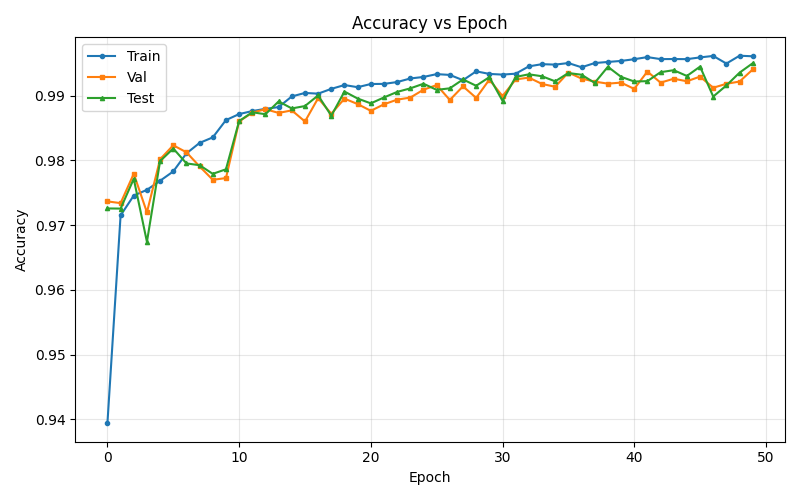
\includegraphics[width=0.85\linewidth]{img/07_analiza_wynikow_i_dzialanie_systemu/plot_accuracy.png}
 \caption{Wykres metryki Accuracy dla najlepszej wersji modelu (v20)}
 \label{fig:mlflow-accuracy}
\end{figure}

Metryka Accuracy rośnie szybko i stabilizuje się na poziomie powyżej 0{,}99 dla wszystkich podzbiorów. W zadaniu segmentacji binarnej jest to jednak metryka pomocnicza, ponieważ może zawyżać ocenę jakości przy dominacji klasy tła.

\begin{figure}[H]
 \centering
 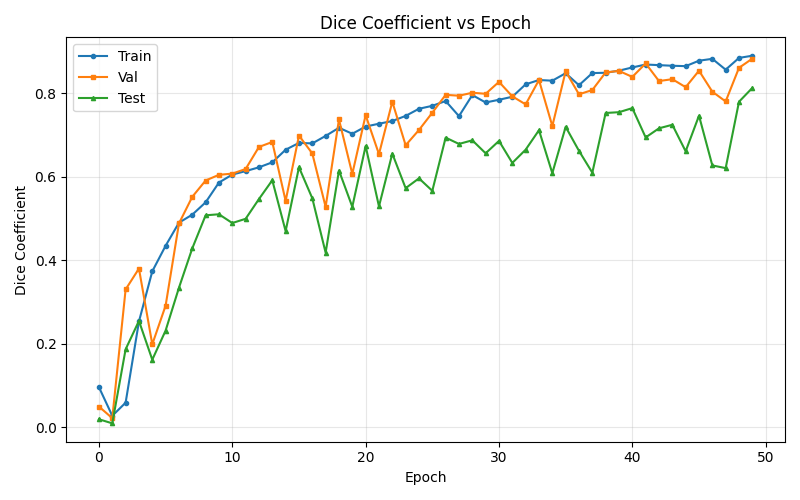
\includegraphics[width=0.80\linewidth]{img/07_analiza_wynikow_i_dzialanie_systemu/plot_dice.png}
 \caption{Wykres metryki Dice dla najlepszej wersji modelu (v20)}
 \label{fig:mlflow-dice}
\end{figure}

Współczynnik Dice, kluczowy dla segmentacji, wykazuje systematyczny wzrost w trakcie uczenia i osiąga wysokie wartości końcowe. Niewielki odstęp między przebiegami treningowym i walidacyjnym wskazuje na dobrą generalizację modelu.

\begin{figure}[H]
 \centering
 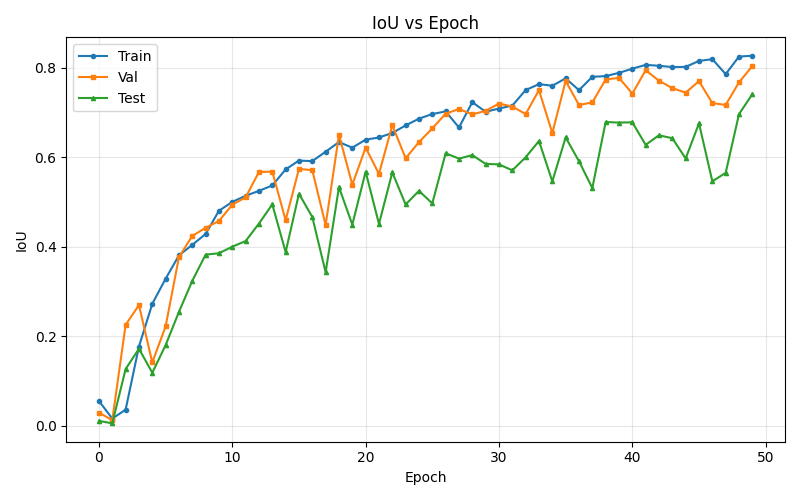
\includegraphics[width=0.85\linewidth]{img/07_analiza_wynikow_i_dzialanie_systemu/plot_iou.png}
 \caption{Wykres metryki IoU dla najlepszej wersji modelu (v20)}
 \label{fig:mlflow-iou}
\end{figure}

Metryka IoU zachowuje trend zgodny z Dice: wyraźnie rośnie wraz z kolejnymi epokami i stabilizuje się pod koniec treningu. Końcowe wartości potwierdzają satysfakcjonującą zgodność predykowanych masek z maskami referencyjnymi.

\begin{figure}[H]
 \centering
 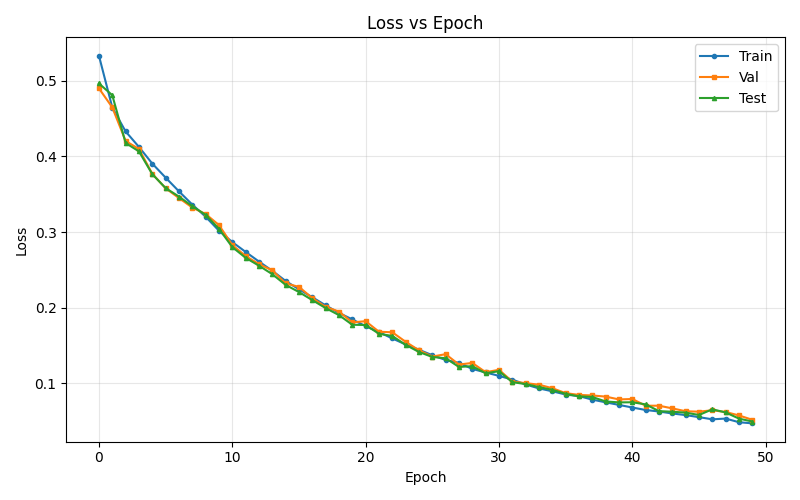
\includegraphics[width=\linewidth]{img/07_analiza_wynikow_i_dzialanie_systemu/plot_loss.png}
 \caption{Wykres funkcji straty dla najlepszej wersji modelu (v20)}
 \label{fig:mlflow-loss}
\end{figure}

Funkcja straty maleje monotonicznie dla zbioru treningowego, walidacyjnego i testowego, bez oznak niestabilności. Taki przebieg potwierdza poprawną zbieżność procesu uczenia i brak wyraźnych symptomów przeuczenia.

\begin{figure}[H]
 \centering
 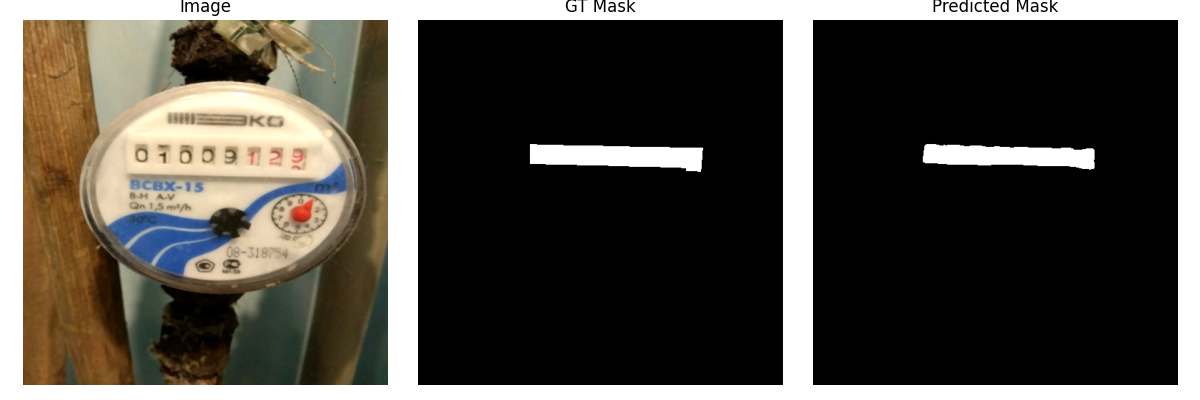
\includegraphics[width=\linewidth]{img/07_analiza_wynikow_i_dzialanie_systemu/plot_pred_2.png}
 \caption{Przykład predykcji modelu v20 (wejście, maska referencyjna, maska przewidywana)}
 \label{fig:mlflow-pred-2}
\end{figure}

\subsection{Koszty infrastruktury}
\label{subsec:koszty}

Analiza kosztowa została zweryfikowana z wykorzystaniem oficjalnego cennika AWS (Price List API) dla regionu \texttt{us-east-1}, stan na luty 2026~\cite{aws_pricing}. Tabela~\ref{tab:koszty-cennik} przedstawia stawki jednostkowe użyte do obliczeń.

\begin{table}[H]
\centering
\caption{Stawki jednostkowe AWS użyte w analizie kosztów}
\label{tab:koszty-cennik}
\begin{tabular}{|p{5.2cm}|p{2.1cm}|p{6.7cm}|}
\hline
\textbf{Pozycja} & \textbf{Stawka} & \textbf{Źródło i uwagi} \\
\hline
EC2 \texttt{t3.large} Linux On-Demand & \$0{,}0832/h & AmazonEC2 Price List API, US East (N. Virginia) \\
\hline
EBS \texttt{gp3} & \$0{,}08/GB-mies. & AmazonEC2 Price List API (wolumen systemowy EC2) \\
\hline
S3 Standard storage & \$0{,}023/GB-mies. & AmazonS3 Price List API, pierwszy próg do 50~TB \\
\hline
S3 PUT/COPY/POST/LIST & \$0{,}005/1000 req. & AmazonS3 Price List API \\
\hline
S3 GET/pozostałe & \$0{,}004/10000 req. & AmazonS3 Price List API \\
\hline
ECR private storage & \$0{,}10/GB-mies. & AmazonECR Price List API \\
\hline
\end{tabular}
\end{table}

Do oszacowania kosztu miesięcznego przyjęto realistyczny profil użytkowania środowiska:
\begin{itemize}
  \item 30~GB wolumenu EBS \texttt{gp3} dla instancji,
  \item 20~GB danych i artefaktów w S3,
  \item 1{,}5~GB obrazów kontenerowych w ECR,
  \item 5000 operacji S3 typu PUT/LIST i 30000 operacji GET miesięcznie,
  \item pojedynczy cykl treningowy: 3{,}5~h pracy EC2.
\end{itemize}

Koszt pojedynczego cyklu obliczeniowego wynosi:
\[
C_{cykl} = 3{,}5 \cdot 0{,}0832 = 0{,}2912\ \text{USD}.
\]

Koszt stały miesięczny (niezależny od liczby cykli) wynosi:
\[
C_{stały} = 30\cdot0{,}08 + 20\cdot0{,}023 + 1{,}5\cdot0{,}10 + \frac{5000}{1000}\cdot0{,}005 + \frac{30000}{10000}\cdot0{,}004 \approx 3{,}05\ \text{USD/mies.}
\]

Całkowity koszt miesięczny można więc zapisać jako:
\[
C_{mies}(N)=3{,}05 + 0{,}2912\cdot N,
\]
gdzie \(N\) oznacza liczbę pełnych cykli treningowych w miesiącu.

\begin{table}[H]
\centering
\caption{Koszt miesięczny dla różnych intensywności użycia pipeline CI/CD}
\label{tab:koszty-scenariusze}
\begin{tabular}{|c|c|c|}
\hline
\textbf{Liczba cykli/mies.} & \textbf{Koszt zmienny EC2} & \textbf{Koszt całkowity} \\
\hline
10 & \$2{,}91 & \$5{,}96 \\
\hline
30 & \$8{,}74 & \$11{,}79 \\
\hline
60 & \$17{,}47 & \$20{,}52 \\
\hline
\end{tabular}
\end{table}

\textbf{Koszt wdrożenia automatyzacji i porównanie z obsługą manualną (PLN).}
Do analizy doliczono jednorazowy koszt przygotowania infrastruktury automatycznej:
\[
C_0 = 10000\ \text{PLN}.
\]

W podejściu manualnym przyjęto, że utrzymanie procesu zajmuje \textbf{20\% czasu pracy inżyniera} (0,2 etatu). Dla miesięcznej pensji brutto \(P\) koszt pracy manualnej wynosi:
\[
C_{\text{manual,praca}} = 0{,}2\cdot P.
\]

Z pomiarów czasu (5 h manualnie vs 20 min w CI/CD) wynika, że obciążenie człowieka po automatyzacji to około \(6{,}67\%\) obciążenia manualnego. Stąd:
\[
C_{\text{CI/CD,praca}} \approx 0{,}0133\cdot P.
\]

Miesięczna różnica kosztu pracy:
\[
\Delta C_{\text{praca}} = (0{,}2 - 0{,}0133)\cdot P = 0{,}1867\cdot P.
\]

Czas zwrotu jednorazowego kosztu wdrożenia:
\[
T_{\text{BE}} = \frac{C_0}{\Delta C_{\text{praca}}}
= \frac{10000}{0{,}1867\cdot P}\ \text{[mies.]}.
\]

\begin{table}[H]
\centering
\caption{Próg opłacalności automatyzacji dla różnych pensji miesięcznych}
\label{tab:break-even-pln}
\begin{tabular}{|c|c|c|c|}
\hline
\textbf{Pensja \(P\) [PLN/mies.]} & \textbf{Manual \(0{,}2P\)} & \textbf{CI/CD \(0{,}0133P\)} & \textbf{Zwrot \(T_{\text{BE}}\)} \\
\hline
8000  & 1600 PLN/mies. & 106 PLN/mies. & 6{,}69 mies. \\
\hline
12000 & 2400 PLN/mies. & 160 PLN/mies. & 4{,}46 mies. \\
\hline
16000 & 3200 PLN/mies. & 213 PLN/mies. & 3{,}35 mies. \\
\hline
\end{tabular}
\end{table}

Wniosek z tej części analizy: nawet po doliczeniu jednorazowego kosztu 10000 PLN automatyzacja zwraca się względnie szybko względem stałego obciążenia pracy manualnej.

Wyniki pokazują, że automatyzacja CI/CD faktycznie przyspiesza pracę i redukuje nakład operacyjny człowieka, ale odbywa się to kosztem stałych i narastających kosztów chmurowych. W praktyce oznacza to, że podejście CI/CD jest \textbf{szybkie i efektywne operacyjnie}, lecz \textbf{kosztowne finansowo} przy większej liczbie iteracji oraz przy przejściu do architektury produkcyjnej o wyższych wymaganiach dostępności i bezpieczeństwa.

\subsection{Zużycie zasobów i działanie usługi}
\label{subsec:zasoby}

Serwis inferencyjny działa stabilnie na instancji \texttt{t3.large}. Model ładowany jest jednorazowo przy starcie kontenera, a monitorowane metryki API (liczba predykcji, opóźnienia, błędy) potwierdzają poprawne działanie wdrożenia. Dla przyjętej skali obciążenia zasoby CPU i RAM były wystarczające.

W kontekście obciążenia należy podkreślić, że projekt był testowany w skali laboratoryjnej, a nie pod pełnym ruchem produkcyjnym. Oznacza to, że sekcja zasobowa potwierdza wystarczalność środowiska dla przyjętego scenariusza, ale nie stanowi pełnego wyznacznika wydajnościowego dla skali wielokrotnie większej.

\subsection{Ocena jakościowa procesu}

\subsubsection{Łatwość wdrożenia}

Konfiguracja systemu wymagała jednorazowego, istotnego nakładu pracy: przygotowania Terraform, konfiguracji k3s i Helm, integracji MLflow z S3, implementacji walidacji danych i bramki jakości oraz przygotowania workflow GitHub Actions. Po wykonaniu tej inwestycji wejściowej kolejne iteracje procesu są realizowane z minimalną interwencją operatora.

Podejście ręczne nie ma kosztu wejścia na poziomie automatyzacji, ale generuje koszt powtarzalny przy każdym cyklu. Wraz ze wzrostem liczby iteracji rośnie obciążenie inżyniera oraz ryzyko błędu ludzkiego.

\subsubsection{Stabilność i podatność na błąd}
\label{subsubsec:stabilnosc}

W podejściu zautomatyzowanym trzy elementy istotnie ograniczają ryzyko błędu ludzkiego:
\begin{itemize}
  \item automatyczna walidacja danych wejściowych przed treningiem,
  \item automatyczna bramka jakości blokująca regresję modelu,
  \item automatyczne zatrzymanie EC2 po zakończeniu pipeline'u (także po błędzie).
\end{itemize}

W podejściu ręcznym wszystkie trzy decyzje pozostają po stronie operatora, co zwiększa prawdopodobieństwo przeoczeń i kosztownych pomyłek.

\begin{table}[H]
\centering
\caption{Porównanie ryzyka operacyjnego: manual vs CI/CD}
\label{tab:ryzyko-porownanie}
\begin{tabular}{|p{4.3cm}|p{5.1cm}|p{5.1cm}|}
\hline
\textbf{Obszar ryzyka} & \textbf{Podejście ręczne} & \textbf{CI/CD} \\
\hline
Walidacja danych & zależna od dyscypliny operatora, ryzyko pominięcia błędnych próbek & automatyczna bramka QA blokująca dalszy pipeline \\
\hline
Decyzja o promocji modelu & ręczna interpretacja metryk, podatność na presję czasu & obiektywne kryterium bramki jakości (Dice/IoU) \\
\hline
Koszt chmury po awarii procesu & ryzyko pozostawienia uruchomionej instancji & automatyczne \texttt{stop-infra} po błędzie (\texttt{always()}) \\
\hline
Odtwarzalność eksperymentu & wymaga ręcznej dokumentacji i dyscypliny & logi workflow + MLflow + DVC zapewniają ślad audytowy \\
\hline
\end{tabular}
\end{table}

\subsubsection{Skalowalność}
\label{subsubsec:skalowalnosc}

Najważniejsza przewaga automatyzacji dotyczy skalowalności pracy zespołu: wzrost liczby iteracji nie zwiększa nakładu pracy człowieka proporcjonalnie do liczby cykli. Ograniczenia obecnej implementacji (single-node k3s, jeden runner, środowisko AWS Academy) mają charakter infrastrukturalny i budżetowy, nie logiczny. Logika pipeline'u może być przeniesiona do większego środowiska bez zmiany modelu procesu.

\begin{table}[H]
\centering
\caption{Skalowalność nakładu pracy człowieka przy wzroście liczby cykli}
\label{tab:skalowalnosc-pracy}
\begin{tabular}{|c|c|c|}
\hline
\textbf{Liczba cykli / mies.} & \textbf{Manual (5 h/cykl)} & \textbf{CI/CD (20 min/cykl)} \\
\hline
10 & 50 h & 3 h 20 min \\
\hline
30 & 150 h & 10 h \\
\hline
60 & 300 h & 20 h \\
\hline
\end{tabular}
\end{table}

Zestawienie to pokazuje, że przy wzroście liczby iteracji różnica obciążenia człowieka rośnie liniowo i szybko staje się kluczowym argumentem organizacyjnym na rzecz automatyzacji.
